\chapter{Partículas Cargadas}

\section{Dispersión de Rutherford}

\subsection{Introducción}

Rutherford describió la dispersión de una partícula $\alpha$ por núcleos atómicos (con $m_\alpha \ll M, z=2$) sobre una trayectoria hiperbólica a través del potencial de Coulomb. La energía total viene dada como la suma de la energía cinética y potencial, y permanece \textit{constante} sobre toda la trayectoria:

\begin{equation}
    E(r) = E_K(r) + E_p (r) \qquad  E_p (r) = \frac{ z Z e^2}{4\pi \varepsilon_0} \frac{1}{R} \qquad E_K (r) = \frac{1}{2} m_\alpha v_\alpha^2
\end{equation}
La distancia de máxima aproximación se define como la distancia a la cual se para una partícula con parámetro de impacto $b=0$, i.e. colisión frontal. Así, denotando $E_K$ como la \textit{energía cinética inicial}, tenemos que

\begin{equation}
   E_K = \frac{zZe^2}{4\pi\varepsilon_0} \frac{1}{D_{\alpha-N}}
\end{equation}
aunque lógicamente esta expresión no será del todo cierta, ya que el potencial no es infinito en $r=0$, debido a que el núcleo es finito. Aún así es una buena aproximación.


\subsection{Relación entre el parámetro de impacto y el ángulo de dispersión}

El momento transferido en la interacción, siempre y cuando $|\pn_i |= |\pn_f|=p$ vale 

\begin{equation}
    \Delta p = 2 p \sin (\theta/2)
\end{equation}
siendo $\theta$ el \textbf{ángulo de dispersión}. Es fácil de deducir matemáticamente, pero incluso físicamente tiene sentido: cuando $\theta=\pi$ la trasferencia de momento es máxima (la partícula se da la vuelta completamente) lo que implicla un intercambio de $2$ veces el momento inicial. Definimos como \textbf{parámetro de impacto} 

\begin{equation}
    b = r \sin \theta
\end{equation}
cuando la partícula está en el infinito. Además, también se conserva el momento angular $L = |\rn \times \pn|=L p \sin \theta$, lo que lleva a la relación 

\begin{equation}
    v_i b = \omega r^2
\end{equation}
siendo $\omega=\dv{\phi}{t}$ en el vértice, definiendo $\phi$ como el ángulo entre el vértice y la partícula desde el núcleo. En el vértice, que es el punto en el cual la posición respecto el átomo y el momento lineal de la partícula son perpendiculares. Tenemos que en el infinito

\begin{equation}
    L_\infty = |\rn \times \pn | = m_\alpha b v_i        
\end{equation}
mientras que en el vértice: 

\begin{equation}
    L_a = |\rn \times \pn | = r p \sin 90^\circ = r m_\alpha \left( r \dv{\phi}{t} \right)  = m_\alpha \omega r^2
\end{equation}  
El momento transferido $\Delta p$ se calcula como la acción total en el tiempo de la fuerza de Coulomb proyectada sobre el eje de la hipérbola, tal que

\begin{equation}
    \Delta p = \int_{-\infty}^{\infty} F_{\Delta p} \D t  = A \int_{-\frac{\pi-\theta}{2}}^{\frac{\pi-\theta}{2}} \frac{\cos \phi}{r^2} \pqty{\dv{t}{\phi} \D \phi}  = \frac{A}{b v_i} \int_{-\frac{\pi-\theta}{2}}^{\frac{\pi-\theta}{2}} \cos \phi \D \phi = \frac{2 A}{v_i b} \cos (\theta/2) \quad A = \frac{zZe^2}{4\pi \varepsilon_0}
\end{equation}
de lo que se puede deducir que el parámetro de impacto $b$ y el ángulo de dispersión se relacionan tal que:

\begin{equation}
    b = \frac{1}{2} D_{\alpha - N} \cot (\theta/2) = \frac{1}{2} D_{\alpha-N} \sqrt{\frac{1+\cos \theta}{1-\cos \theta}} \qquad D_{\alpha-N} = \frac{zZe^2}{4\pi \varepsilon_0} \frac{1}{E_K}
\end{equation}
siendo $\D_{\alpha-N}$ la distancia de máxima aproximación y $E_K$ la energía cinética. 

\subsection{La sección eficaz diferencial de Rutherford}

La dispersión de las partículas alfa que halló Rutherford la describió en función de su sección diferencial, tal que:

\begin{Resalte}
\begin{equation}
    \dv{\sigma_{\Ruth}}{\Omega} =  \pqty{\frac{D_{\alpha-N}}{4}}^2 \frac{1}{\sin^4 \frac{\theta}{2}} \qquad D_{\alpha-N} = \frac{zZe^2}{4\pi\varepsilon_0} \frac{1}{E_K}
\end{equation}
\end{Resalte}
Esta ecuación, aunque fue calculado con la mecánica clásica, también puede ser hallada en la mecánica cuántica, usando las aproximaciones de Born a primer orden ya vistas. 
 
Como podemos comprobar, \textit{diverge} para $\theta=0$, lo cual es debido al carácter ideal del núcleo puntual. La razón por la que en realidad no diverge, o la solución a esta divergencia, es que la carga nuclear está apantallada por los \textit{electrones orbitales atómicos}, lo que conduce a un ángulo mínimo $\theta_{\min}$. La dispersión hacia atrás ($\theta \to \pi, b \to 0$) tampoco se logra nunca, debido al radio finito del núcleo. 

En ambos casos el punto es el mismo: debido a la localización de la partícula al interaccionar con el potencial, el propio principio de incertidumbre genera un $\Delta p$ relacionado directamente con el rango efectivo del potencial $x$, tal que

\begin{equation}
\Delta p \approx \frac{\hbar}{x}
\end{equation}
y, debido a esto y la geometría, el ángulo medio 
\begin{equation}
    \bar{\theta} = \frac{\Delta p}{p} 
\end{equation}
que se puede ver geométricamente. De todos modos tampoco hace falta entenderlo físicamente, basta con ver que las correciones físicamente correctas al potencial de Coulomb (al no ser, los átomos, ``objetos cargados'', ni los núcleos ``cargas puntuales'') basta para ver que aparecen un ángulo mínimo y máximo.

\subsection{Ángulo mínimo: corrección por apantallamiento}
Un modelo que tiene en cuenta el apantallamiento es el \textit{modelo atómico estadístico de Fermi}, el cual introduce una exponencial tabulada por un \textit{radio efectivo} $\alpha_{TF}$ de tal modo que el potencial de Coulomb no caiga ``lentamente''. Así pues: 

\begin{equation}
    V_{TF} (r) = \frac{zZe^2}{4\pi\varepsilon_0} \frac{1}{r} e^{-\frac{r}{a_{TF}}}
\end{equation}
el \textit{radio efectivo} $a_{TF}$ de la nube electrónica (de Thomas-Fermi) decrece por debajo del radio de Bohr $\alpha_0$ al aumentar $Z$, como $a_{TF}=\frac{\zeta a_0}{\sqrt[3]{Z}}$, debido a la disminución del tamaño de los orbitales más internos, por el teorema de Gauss. 

La aproximación de Born requiere ahora, con $\Delta k = K=(2p/\hbar) \sin(\theta/2) (p=p_i)$ el momento de onda transferido ($p = \hbar k$), el cálculo de la transformada seno de $V_{TF}(r)$, que es finita. Rutherford reciba entonces un \textit{factor corrector} tal que:

\begin{equation}
    \dv{\sigma_{\Ruth}}{\Omega} = \vqty{\frac{2m_\alpha}{\hbar^2}\int_{0}^{\infty} r^2 V_{TF}(r) \frac{\sin Kr}{Kr} \D r }^2 = \pqty{\frac{D_{\alpha-N}}{4}}^2 \frac{1}{\sin^4 \theta/2} \pqty{\frac{1}{1+\frac{1}{K^2 a_{TF}^2}}}
\end{equation}
Cuando $\theta\ll 1$, tenemos que: 

\begin{equation}
    \dv{\sigma_{\Ruth}}{\Omega} = \frac{D_{\alpha-N}^2}{\theta^4} \frac{1}{\bqty{1+\pqty{\frac{\theta_{\min}^2}{\theta^2}}^2}} = \frac{D_{\alpha-N}^2}{\theta^2+\theta_{\min}^2} 
\end{equation}
donde se introduce el concepto el concepto de ángulo mínimo, que como podemos ver viene expresado: 

\begin{equation}
    \theta_{\min} = \frac{\hbar}{p a_{TF}} = \frac{\hbar \sqrt[3]{Z}}{pa_{TF}} = \frac{\hbar c \sqrt[3]{Z}}{a_0 \sqrt{E_K(E_K+2Mc^2)}}  \label{Ec:02-thetamin}
\end{equation}
donde hemos usado que 

\begin{equation*}
    p^2 c^2 = E^2 - m^2 c^4 \Rightarrow p  = \frac{1}{c} \sqrt{E^2 - m^2 c^4 - M^2 c^4} = \frac{1}{c} \sqrt{(E_K + m c^2 + M c^2)^2 - m^2 c^4  - M^2 c^4} 
\end{equation*}
que despreciando la masa de la partícula incidente $m$ frente a $M$
\begin{equation}
    p  \approx \frac{1}{c} \sqrt{E_K (E_K + 2 Mc^2) } 
\end{equation}
La mejora de la aparición de este ángulo mńimo es que ahora \textit{la sección eficaz total es finita}, lo cual se corresponde a un resultado mucho más físico. Este ángulo mínimo tiene un \textit{origen cuántico} debido al \textit{principio de incertidumbre}. Se produce por la localización de la partícula sobre el radio $a_{TF}$, que le imprime un momento \textit{transversal} inevitable $\Delta p$, relacionado con la longitud de onda: 
\begin{equation}
    \theta_{\min} = \frac{\Delta p}{p} \approx \frac{\hbar}{pa_{TF}} = \frac{\lambdabar}{a_{TF}}
\end{equation}
\subsection{Ángulo máximo: corrección por radio finito del núcleo}

El potencial que ve una carga elemental $z$ cerca del núcleo $V(r)$ tiene un plateu en su interior hasta $r=R$ y para $r>R$ adopta la forma de Coulomb $E_p(r)$. Una forma de representar  este potencial es con la ecuación 

\begin{equation}
    V_{FSN} (r) = \frac{zZe^2}{4 \pi \varepsilon_0} \frac{1}{r} \pqty{1-e^{-\frac{2r}{R}}}
\end{equation}
en la \cref{Fig:02.01} vemos la representación de esta función. 

\begin{figure}[H] \centering
    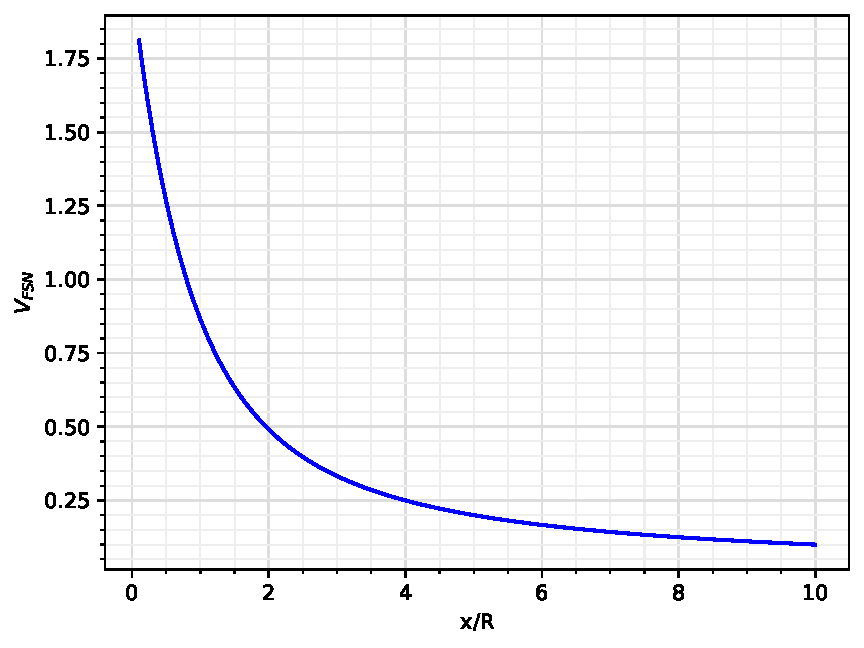
\includegraphics[width=0.6\linewidth]{Images/Ch_02/02-Vfsn.pdf}
    \caption{Representación del potencial $V_{FSN}(r)$. Como podemos comprobar no representa un ``plateu'', pero tampoco hace infinito al potencial en el centro, lo que nos basta.}
    \label{Fig:02.01}
\end{figure}

La nueva expresión de la sección eficaz de Rutherfrod con este potencial vendrá dada por:

\begin{equation}
    \dv{\sigma_{\Ruth}}{\Omega} = \pqty{\frac{D_{\alpha-N}}{4}}^2 \frac{1}{\sin^4(\theta/2)} \frac{1}{\bqty{1+\pqty{\frac{\sin (\theta/2)}{\bar{\theta_{\max}}}}^2}^2}
\end{equation}
Siendo $\bar{\theta_{\max}}$ un parámetro de origen cuántico que suprime la probabilidad de dispersión hacia atrás, siendo solo significativa para $0<\theta<\theta_{\max}<\pi$. Toma el valor:

\begin{equation}
    \bar{\theta}_{\max} = \frac{\hbar}{p R} = \frac{\hbar }{R_0 \sqrt[3]{A} \sqrt{E_K (E_K+Mc^2)}}   \label{Ec:02-tehtamax}
\end{equation}
Ilustra las fluctuaciones transversales que impiden la localización de la hipérbola clásica hacia atrás. 


\section{Dispersión de Mott} 

La dispersión de Mott tiene básicamente 3 correcciones: la correción relativista, es decir, la correción que se hace a la energía y momento cuando partícula tiene una energía cinética inicial de entorno la masa de la partícula; la correción por el espín (para partículas muy relativistas) y la corrección por el retroceso del núcleo (que se da cuando la partícula no tiene una gran masa respecto la de la partícula incidnete). En el marco de la física médica estas tres son suficientes. 

\subsection{Correcciones relativistas}

La correción relativista (aunque no ultrarrelativista) implica el simple intercambio de  $2E_K = p v = m \gamma \beta^2  c^2$, es decir, multiplicar por $\gamma$: 

\begin{equation}
    D_{n-N}  = \pqty{\frac{zZe^2}{4\pi\varepsilon_0}} \frac{1}{\frac{1}{2}m_n \gamma c^2 \beta^2}
\end{equation}
Aunque ahora $D_{n-N}$ no se llama distancia de máxima aproximación, sino \textit{distancia característica efectiva.}


\subsection{Correcciones por espín}

La correción por el espín está relacionada con la \textit{helicidad} $h$, que se define como la proyección del momento sobre el espín: 

\begin{equation*}
    h = \frac{\sn \cdot \pn}{|\sn||\pn|}
\end{equation*}
Este se conserva edebido a la forma de los espinores en el sistema centro de masas cuando tenemos partículas ultrarrelativistas. Un intercambio de dirección del momento sin modificar también la dirección del espín implicaría que se violaría paridad, lo que no puede ocurrir. Esto es lo que expresa el factor: 

\begin{equation}
    f_{\text{espin}} = 1 - \beta^2 \sin^2 (\theta/2) \to \frac{1}{2} \pqty{1+\cos \theta}
\end{equation}
tal que: 

\begin{equation}
    \dv{\sigma_{\text{Mott}}}{\Omega} =  \dv{\sigma_{\Ruth}}{\Omega}  f_{\text{espin}}
\end{equation}
aunque aún queda una corrección. 



\subsection{Correcciones por retroceso del núcleo}

La correción por retroceso del núcleo está relacionada con la asunción de que el núcleo tiene una masa infinita, por lo que no adquire momento y la colisión es totalmente elástica. Sin embargo, si hay un momento transferido $\Delta p$ le imprime cierta energía cinética al núcleo: $\Delta E = {\frac{\pqty{\Delta p}^2}{2M}} = E_K'-E_K$, tal que $p_f\neq p_i$. Como hemos visto, ahora tenemos que tener en cuenta el factor $p'/p$ en la expresión de la sección eficaz, debido al cambio en el espacio de fases, tal que

\begin{equation}
    \dv{\sigma_{\text{Mott}}}{\Omega} = f_{\text{espin}}f_{\text{retroceso}} \dv{\sigma_{\Ruth}}{\Omega}  
\end{equation}
siendo 

\begin{equation}
    f_{\text{retroceso}} = \frac{p'}{p} 
\end{equation}
que en el caso relativista: 

\begin{equation}
    f_{\text{retroceso}} = \frac{p'}{p}  \approx  \frac{E_K'}{E_K}    
\end{equation}
Veamos como se llegan a ellas: 

\begin{equation}
    E_K' = E_K - \Delta E \quad E_K^2 = p^2 c^2 + m_e^2 c^4 \quad \Delta E = {\frac{\pqty{\Delta p}^2}{2M}} \approx \frac{1}{2M} 4 p^2 \sin^2 (\theta/2) = \frac{E_K^2-m_e^2c^4}{2Mc^2} 2 \sin^2 (\theta/2)
\end{equation}
donde hemos usado que $\Delta p^2 = 4 p^2 \sin^2 (\theta/2)$. Esto nos lleva a que:

\begin{equation*}
    \Delta E \approx \frac{E_K^2}{Mc^2} \sin^2 (\theta /2) \Longrightarrow
\end{equation*}
\begin{equation} E_K ' = E_K  \pqty{1 - \frac{E_K}{Mc^2} 2 \sin^2 (\theta/2)} = E_K \pqty{1 - \frac{E_K}{Mc^2} (1  - \cos^2 (\theta) )} \approx \frac{1}{1+\pqty{\frac{E_K}{Mc^2} (1  - \cos^2 (\theta) )}}
\end{equation}
y, consecuentemente, a que el factor de correción por retroceso sea

\begin{equation}
    f_{\text{retroceso}}  = \frac{1}{1+\pqty{\frac{E_K}{Mc^2} (1  - \cos^2 (\theta) )}}
\end{equation}


\subsection{Correcciones por factor de forma nuclear}

El factor de forma nuclear se relaciona con la densidad de carga (distribución de carga) dentro del núcleo, tal que $f(k)$ es :

\begin{equation}
    f(k) = \int_{\text{nucleo}} \rho (\rn) e^{-i \kn \cdot \rn} \D^3 \rn
\end{equation}
tal que la sección eficaz experimental real: 

\begin{equation}
     \dv{\sigma_{\text{exp}}}{\Omega} =  |f_{k}|^2 \dv{\sigma_{\text{Mott}}}{\Omega}
\end{equation}

\section{Dispersiones individuales}
 
La mayor parte e las interacciones de las partículas y la materia se producen como colisiones elásticas de Coulomb con los átomos. Las colisiones o bien pueden ser con los electrones orbitales de los átomos o con el núcleo. En cualquiera de los casos, la trayectoria de las partículas es una hipérbola, aunque en función del signo relativo tendremos que el foco será interior (atractivo) o exterior (repulsivo).

La sección eficaz individual puede escribirse, cuando el ángulo es muy pequeño $(\theta \ll 1)$, cómo: 

\begin{equation}
    \dv{\sigma}{\Omega} = \frac{D_{ab}^2}{\pqty{\theta^2 + \theta_{\min}^2}^2}
\end{equation}
Este ángulo mínimo ya sabemos de donde procede: del apantallamiento de Coulomb de los electrones en los orbitales, y cómo se puede calcular también lo sabemos, dependiendo únicamente de la energía inicial de la partícula, de la carga de la partícula incidente, y de la carga y masa del blanco. En función de $a$ y $b$, esto es, del blanco y partícula incidente, también dependerá  la expresión de $D_{ab}$, tal y como veremos en el siguiente apartado.

\subsection{Clasificación de las colisiones elásticas con la materia}

Aquí podemos ver que principalmente en función de la masa de la partícula (y por ende, de si es relativista o no) tendremos una expresión u otra de la distancia de máxima aproximación/distancia 

\begin{itemize}
    \item Por ejemplo un ion pesado o protón frente a un núcleo. En este caso no suele ser relativista, por lo que la expresión correcta sería
    \begin{equation}
            D_{\alpha-N} = \frac{zZe^2}{4\pi \varepsilon_0} \frac{2}{p_\alpha v_\alpha }
    \end{equation}
    aunque si llegara a ser relativista $p_{\alpha} = m_{\alpha} \gamma_{\alpha} \beta_{\alpha} \beta_{\alpha} c$. 
    \item Cuando hacemos la colisión electrón-núcleo podemos suponer que es siempre relativista (y $z=1$)
    \begin{equation}
            D_{e-N} = \frac{Ze^2}{4\pi \varepsilon_0} \frac{2}{ m_{e} \gamma_{e} \beta_{e}^2 c^2 }
    \end{equation}
    \item Cuando hacemos electrón-electrón orbital: 
    \begin{equation}
            D_{e-e} = \frac{e^2}{4\pi \varepsilon_0} \frac{2}{p_\alpha v_\alpha }
    \end{equation}
    \item Finalmente, cuando hacemos electrón-átomo: 
    \begin{equation}
            D_{e-a} = \sqrt{D_{e-N}^2+ZD_{e-e}^2} = \frac{\sqrt{Z(Z+1)}e^2}{4\pi \varepsilon_0} \frac{2}{\gamma_e m_e \beta^2_e c^2 }
    \end{equation}
\end{itemize}

\subsection{Ángulos de dispersión mínimo y máximo}

Ya hemos revelado como se originan tanto el ángulo mínimo como el ángulo máximo (desviación de la ley de Coulonmb de su carácter puntual), y se corresponden con parámetro de impacto $b \to \infty$ y $b \to 0$ (al final cuando va hacia atrás $b=0$, dispersión frontal, y vicerversa). Recordando la \cref{Ec:02-thetamin} y \cref{Ec:02-tehtamax}, queda claro que el cociente entre $\bar{\theta}_{\max}$ y $\theta_{\min}$, tal que: 

\begin{equation}
    \frac{\bar{\theta}_{\max}}{\theta_{\min}} = \frac{a_F}{R_0 \sqrt[3]{A}} = \frac{a_0}{R_0} \frac{1}{\sqrt[3]{AZ}}  =  \frac{0.423 \times 10^5}{(AZ)^{1/3}} \label{Ec:02-CocienteDeAngulos}
\end{equation}
siendo $a_F$ el radio efectivo del átomo, $a_0$ el radio de Bohr,  y $R_0 \approx 1.2$ fm, que es el tamaño del núcleo de hidrógeno. El comportamiento respecto la energía tanto de $\bar{\theta}_{\max}$ y $\theta_{\min}$ es parecido, ya que ambos dependen del mismo parámetro $p_i$ en el denominador.
Cuando $\bar{\theta_{\max}}>\pi$, se asume que $\theta_{\max} = \pi$, esto es: 

\begin{equation}
    \theta_{\max} = \max \Bqty{\bar{\theta}_{\max}, \pi}
\end{equation}

\subsection{Ángulo cuadrático promedio}

La sección eficaz total es un parámetro muy importante, ya que nos permite hallar cuantas interacciones entre las partículas de un haz incidente y las del blanco material ocurren. Veamos que, si $\theta \ll 1$: 

\begin{equation*}
    \sigma = \int \dv{\sigma}{\Omega} \D \Omega = 2 \pi D \int_0^{\bar{\theta}_{\max}} \frac{\theta   \D \theta}{\pqty{\theta^2 + \theta_{\min}^2}^2} =  2 \pi D \bqty{-\frac{1}{2} \frac{1}{\theta^2 + \theta_{\min}^2}}_{0}^{\theta_{\max}}
\end{equation*}
de lo que se deduce 
\begin{equation}
    \sigma =\pi D^2 \frac{1}{\theta^2_{\min}} \bqty{1-\frac{1}{1+(\theta_{\max}/\theta_{\min})^2}} \approx \frac{\pi D^2}{\theta_{\min}^2}
\end{equation}
(donde hemos usado $\cos \theta \approx \theta$). Ahora, lo sguiente es calcular el \textbf{ángulo cuadrático promedio}, ya que es una medida que nos permite hallar luego el ángulo cuadrático medio para dispersiones múltiples. 

\begin{equation}
    \bar{\theta}^2 = \frac{\int_{0}^{\theta_{\max}} \theta^2  \dv{\sigma}{\Omega} \D \Omega}{\int_{0}^{\theta_{\max}} \dv{\sigma}{\Omega} \D \Omega} = \frac{2\pi D^2}{\sigma} \int_{0}^{\theta_{\max}} \frac{\theta^3 \D \theta}{(\theta^2 + \theta_{\min}^2)^2}
\end{equation}
pudiendo obtener:

\begin{equation}
    \bar{\theta}^2 = \theta_{\min}^2 \bqty{\ln \pqty{1+\frac{\theta^2_{\max}}{\theta^2_{\min}}} - \frac{1}{1+(\theta_{\max}/\theta_{\omega})^2}}  
\end{equation}
dado que $ \frac{\bar{\theta}_{\max}}{\theta_{\min}} \propto a_0 /R_0 \gg 1$, podemos asumir la aproximación: 

\begin{equation}
    \bar{\theta}^2 = \theta_{\min}^2 \ln \pqty{\frac{\theta_{\max}^2}{\theta_{\min}^2}}    \label{Ec:02-AnguloCuadraticoPromedio}
\end{equation}
Si sustituimos $A=2Z$ (y suponemos que $\theta \ll 1, \theta_{\min} \ll \theta_{\max}$ y que $\sigma = \pi D^2 / \theta_{\min}^2$), entonces: 

\begin{equation}
    \bar{\theta}^2 \approx  4 \theta_{\min}^2 \ln \bqty{183 Z^{-1/3}}  \label{Ec:02-AnguloCuadraticoPromedio2}
\end{equation}

\section{Dispersiones múltiples}

Las dispersiones múltiples, a diferencia de las dispersiones individuales, están gobernadas (o mejor dicho, están parametrizadas) en función de: la longitud de radiación $X_0$, el ángulo cuadrático promedio múltiple $\overline{\Theta^2}$, y el poder de dispersión angular másico $T/\rho$. 

\subsection{Ángulo Cuadrático Medio}

Cuando un haz paralelo de partículas incide una lámina, siempre y cuando todos los ángulso de deflexión sean pequeños, podemos obtener un ángulo de desviación cuadrático promedio $\overline{\Theta^2}$. El teorema del límite central (que básicamente habla de como la suma de variables aleatorias procedentes de una misma distribución nos lleva a una gaussiana) nos asegura que 

\begin{equation}
    \overline{\Theta^2} = n \bar{\theta}^2 
\end{equation} 
siendo $n$ el número de colisiones de la partícula (para que esto se cumpla $n>20$).  Vamos a obtener entonces cual es el número de colisiones (promedio) en el absorbente de grosor $t$. Si $\sigma$ es la sección eficaz total

\begin{equation}
    n = \frac{N_a}{V} \sigma t = \rho \frac{N_A}{A} \sigma t \approx \pi \rho \frac{N_A}{A} \frac{D^2}{\theta^2_{\min}} t 
\end{equation}
que si lo juntamos con la \cref{Ec:02-AnguloCuadraticoPromedio} tenemos entonces:

\begin{equation}
    \overline{\Theta^2} = \pi \rho \frac{N_A}{A} D^2 t \ln \pqty{\frac{\theta_{\max}^2}{\theta_{\min}^2}} 
\end{equation}
ahora podemos aplicar la ecuación \cref{Ec:02-CocienteDeAngulos} para poder reexpresar $\overline{\Theta^2}$ en función de $Z$ y $A$, tal que así 

\begin{equation}
    \overline{\Theta^2} = \pi \rho \frac{N_A}{A} D^2 t \bqty{2 \ln \pqty{\frac{a_0}{R_0} \frac{1}{\sqrt[3]{AZ}}}}. 
\end{equation}
que, en función de la partícula incidente y del blanco, siempre podremos aproximar (bien podemos suponer $A \approx 2 Z$, un valor para $a_0$ y $R_0$...). La aproximación usando esto último es (\cref{Ec:02-AnguloCuadraticoPromedio2}) obtenida es: 

\begin{equation}
    \overline{\Theta^2} = 4 \pi \rho D^2 t \frac{N_A}{A} \ln \pqty{183 Z^{-1/3}}
\end{equation}


\subsection{Poder de dispersión angular másico}

La siguiente definción de interés es el \textbf{poder de dispersión angular másico}, qeu se define como

\begin{equation}
    \frac{T}{\rho} = \frac{\overline{\Theta^2}}{\rho t}
\end{equation}
con unidades $[\unit{rad^2 cm^2 /g}]$ ($T [\unit{rad^2 cm^{-1}}]$). 


\subsection{Longitud de radiación}

La longitud de radiación $X_0$ se define como 

\begin{equation}
    \frac{1}{X_0} = 4 \alpha \frac{N_A}{A} Z (Z +1) r_e^2 \ln \pqty{\frac{183}{Z^{1/3}}}
\end{equation}
que es la expresión que surge de \cref{Ec:02-AnguloCuadraticoPromedio2} entre otras. Esta variable representa la distancia promedio que una partícula cargada relativista viaja en el medio para que su enerǵia se reduzca un factor $1/e$ (al 36.8 \%) respecto su valor inicial. También representa 7/8 del camino libre medio necesario para que se emita un par $e^+e^-$. Puede ser una unidad másica si dividimos por la densidad ($\unit{cm^2}/g$), aunque el significado físico se obtiene cuando es una distancia. 


\section{Energía trasferida en choque relativista}

El choque frontar $b=0$ entre un proyectil de masa en reposo $m_1$ y un blanco de masa en reposo $m_2$ produce la máxima energía de trasferencia y el máximo momento trasferido. Para calcularlo tenemos que aplicar las ecuaciones de la \textit{conservación del momento y energía relativista} $p^{\mu}_i = p^{\mu}_f$, tal que 
\begin{equation}
    p_i^\mu = (\gamma m_1c^2+ m_2c^2, \pn_1) \qquad 
    p_f^\mu = (\gamma_1 m_1c^2+ \gamma_2 m_2c^2, \pn_1' + \pn_2')
\end{equation}
De aquí se deducen dos expresiones, la conservación de la energía (primer elemento del cuadrimomento)
\begin{equation}
    \gamma m_1 c^2 + m_2 c^2 = \gamma_1 m_1 c^2 + \gamma_2 m_2 c^2
\end{equation}
y la conservación del momento: 
\begin{equation}
    \pn_1 =  \pn_1' + \pn_2 '
\end{equation}
donde los momentos primados son los momentos tras la colisión. Llamando a $E_{ki}$ la energía cinética inicial ($E_{ki}=(\gamma-1)m_1c^2$) y a $\Delta E$ la trasferencia de energía (que es básicamene la enerǵia cinética de la partícula 2, tal que $\Delta E = (\gamma-1)m_2 c^2)$ podemos deducir no trivialmente la siguiente relación: 

\begin{equation}
    \Delta E_{\max} = \frac{2(\gamma+1)m_1m_2}{m_1^2 + m_2^2 + 2 \gamma m_1 m_2} E_K^i = \frac{2 m_2 c^2 \beta^2 \gamma^2}{1+ 2 \gamma \frac{m_2}{m_1} + \pqty{\frac{m_2}{m_1} }^2}
\end{equation}
la segunda expresión es la que más podemos encontrar en la literatura, como por ejemplo en la pág. 3 \cite{PDG2020_Passage}. En el ejercicio \ref{Ej:02.02} proponemos llegar a estas expresiones con las definiciones dadas aquí. Luego además tenemos la máxima transferencia de momento: 

\begin{equation}
    \Delta p_{\max} = \frac{2(m_1\gamma+m_2)m_2}{m_1^2 + m_2^2 + 2 \gamma m_1 m_2} p_i 
\end{equation}
Lógicamente se suelen usar aproximaciones en función de los casos que facilitan las expresiones analíticas. Los casos más generales son: 

\begin{itemize}
    \item Caso $m_2 \ll m_1$. En este caso, sencillamente aplicamos la expresión 
    \begin{equation}    
        \Delta E_{\max} =\frac{2 m_2 c^2 \beta^2 \gamma^2}{1+ 2 \gamma \frac{m_2}{m_1} + \pqty{\frac{m_2}{m_1} }^2} \approx  2 m_2 c^2 \beta^2 \gamma^2 \approx 2 m_2 c^2  \pqty{\frac{\beta^2}{1-\beta^2}}
    \end{equation}
    y si queremos obtener el caso no relativista ($\beta \to 0$) tenemos que
    \begin{equation}
        \Delta E_{\max} \approx 2 m_2 v^2 
    \end{equation}
    siendo $v$ la velocidad inicial de la partícula incidente ($v=\beta c$).
    \item Caso $m_2 \gg m_1$
    \begin{equation}
        \Delta E  =\frac{2 m_2 c^2 \beta^2 \gamma^2}{1+ 2 \gamma \frac{m_2}{m_1} + \pqty{\frac{m_2}{m_1} }^2}  \approx   \frac{2m_1c^2 \beta^2 \gamma^2}{2\gamma + \frac{m_2}{m_1}} \pqty{\frac{\beta^2}{1-\beta^2}}
    \end{equation}
    de nuevo, si nos alejamos del gaso relativista $\gamma \to 1, \beta \to 0$, tenemos:
    \begin{equation}
        \Delta E = 2 \frac{m_1^2}{m_2} v^2  = 4 \frac{m_1}{m_2} E_k
    \end{equation}
    \item Caso $m_2 = m_1$ y además partículas distinguibles.
    \begin{equation}
        \Delta E = \frac{2(\gamma+1)m_1m_2}{m_1^2 + m_2^2 + 2 \gamma m_1 m_2} E_K^i = E_K^i
    \end{equation}
    \item Caso $m_2 = m_1$ y además partículas indénticas.
    \begin{equation}
        \Delta E = \frac{E_K^i}{2} 
    \end{equation}
    esto se debe a que al ser las dos posibles partículas incidentes (son indistiguibles) debemos reducir la expresión a la mitad (mecánica estadística).
\end{itemize}
Existe un parámetro, llamado \textbf{fracción de energía máxima trnasferida} 

\begin{equation}
    \eta = \pqty{\frac{\Delta E_{\max}}{E_K}} 
\end{equation}
A valores muy altos de $E_K$ se transifere toda la energía del proyectil al blanco. En el caso de partículas de la misma y distinguibles la energía transferida es del 100\%, y si son indistiguibles del 50\%.

\section{Poder de frenado másico}



\subsection{Definición}

\subsection{Poder de frenado másico por radiación}


\subsection{Poder de frenado másico por colisión}


\subsection{Teoría de Bethe del frenado másico por colisión}

\subsection{Correciones de Bethe y extensión al electrón y positrón}

\subsection{Balance entre colisión y radiación: energía crítica}


\section{El rango másico $R_{CSDA}$}

Al atraversar un medio las partículas cargadas experimentan deflexiones respecto a su camino original, debido a las colisiones tanto ionizantes como elásticas. Estos efectos son mucho más pronunciados para electrones, que además sufrer colisiones radiativas con emisión de fotones. Para describir la \textit{longitud promedio que la partícula penetra en el absorbente} hasta pararse se usa el \textbf{rango en la aproximación de frenado continuo} $R_{CSDA}$, tal que 

\begin{equation}
    R_{CSDA} \equiv \int_{0}^{E_K^0} \frac{\D E }{S_{tot}(E) } \qquad [\unit{g \ cm^{-2}}]
\end{equation}



\section*{Ejercicios}
\addcontentsline{toc}{section}{Ejercicios}




\begin{Ejercicio}{Sección eficaz de Rutherford con modelo atómico de Fermi} \label{Ej:02.01}
    Obten la expresión de la sección de eficaz de Rutherford, ahora con el potencial del modelo atómico estadístico de Fermi, usando la aproximación de Born con ondas planas incidentes y salientes

    \begin{equation*}
        \dv{\sigma_{\Ruth}}{\Omega} =  \pqty{\frac{D_{\alpha-N}}{4}}^2 \frac{1}{\sin^4 \theta/2} \pqty{\frac{1}{1+\frac{1}{K^2 a_{TF}^2}}}
    \end{equation*}
    y luego llegar a la expresión final cuando $\theta\ll 1$: 
\end{Ejercicio}

\begin{Ejercicio}{$\Delta E_{\max}$ y $\Delta p_{\max}$ en colisión con blanco fijo.} \label{Ej:02.02}
    A partir de la conservación del cuadrimomento $p^{\mu}_i = p^{\mu}_f$ encuentra la expresión de máxima trasnferencia de la energía y del momento $\Delta E_{\max}$ y $\Delta p_{\max}$. 
    \begin{equation}
        \Delta E_{\max} = \frac{2(\gamma+1)m_1m_2}{m_1^2 + m_2^2 + 2 \gamma m_1 m_2} E_K^i \qquad 
        \Delta p_{\max} = \frac{2(m_1\gamma+m_2)m_2}{m_1^2 + m_2^2 + 2 \gamma m_1 m_2} p_i 
    \end{equation}
    Véase la solución en \cite{Montaruli201x_Exercise4}.
\end{Ejercicio}

\begin{Ejercicio}{Transferencia de momento y energía por partículas cargadas} \label{Ej:02.03}

Recuerda las relaciones obtenidas para la transferencia $\Delta p$ y $\Delta E$ en una colisión a través de la ley de Coulomb entre una partícula pesada de masa $M$ y carga $+Ze$ y un electrón orbital (carga $-e$ y masa $m_e$), con un valor fijo del parámetro de impacto $b$, teniendo en cuenta las leyes de conservación de $p$, $E$, y del momento angular $L$. En dicha colisión clásica y no relativista, el electrón orbital se sitúa en el foco interno de una hipérbola. Si la partícula cargada es pesada tenemos $M \gg m_e$ y el ángulo de dispersión es nulo $\theta \approx 0$, entonces:

\[
\Delta p(b) = \frac{2 Z r_e m_e c^2}{v b}, \qquad 
\Delta E(b) = \frac{(\Delta p)^2}{2 m_e} = \frac{2 Z^2 r_e^2 m_e c^2}{(v/c)^2 b^2}, \qquad
b = \frac{2 Z r_e m_e c^2}{v \Delta p} = \frac{Z r_e (v/c)}{\sqrt{2 m_e c^2 / \Delta E}}
\]

\begin{enumerate}[label=\alph*)]
\item Tanto $\Delta p$ como $\Delta E$ tienen un valor mínimo y un valor máximo. Recuerda cuál es su fundamento, y determina ambos en cada caso $\Delta p_{\min,\max}$ (en KeV/c) y $\Delta E_{\min,\max}$ (en eV), para un \emph{protón} incidente de energía cinética $E_K = 10$ MeV, añadiendo 4 filas más al Cuadro 3, cada una con los 7 elementos.

\item  Debido a su dependencia con el parámetro de impacto $b$, tenemos también un valor mínimo y máximo de éste. Añade al Cuadro 3 los valores de $b_{\min}$ y $b_{\max}$ (en fm) en dos nuevas filas. ¿Es posible la colisión entre una partícula cargada pesada y un electrón orbital del absorbente, estando el parámetro de impacto fuera del rango $b \in (b_{\min}, b_{\max})$? Discute por separado los casos $b > b_{\max}$ y $b < b_{\min}$, intentando caracterizarlos físicamente, si crees que aún son posibles. Aclara el marco de la aproximación realizada en la derivación de las fórmulas anteriores, especialmente para el segundo caso. ¿Son siempre elásticas las colisiones del proyectil con los \emph{núcleos atómicos}? \\[1em]
\end{enumerate}

\begin{center}
\begin{tabular}{lcccccccccccccccccccccccccccc}
\toprule & H & Al & Cu & Ag & Au & Tl & Pb \\
\midrule
Número atómico $Z$ & 1 & 13 & 29 & 47 & 79 & 81 & 82 \\
Potencial de ionización / excitación $I$ (eV) & 19 & 166 & 322 & 470 & 790 & 727 & 823 \\
\bottomrule
\end{tabular}
\end{center}
\end{Ejercicio}

\begin{enumerate}[label=\alph*)]
    \item Suponiendo un protón incidente con una energía cinética de $E_K=10$ MeV, tal que $E_K\ll m_p c^2$ y por tanto el momento inicial aproximable a la relación clásica:

    \begin{equation*}
        p_i \approx \sqrt{2 m_p E_K} =  \qquad v_i = \frac{p_i}{m_p} = 
    \end{equation*}
    El momento máximo y la energía máxima transferibles, dado que estamos en una colisión no relativista, vienen dados por (básicamente $\gamma \to 1$ en las ecuaciones ya vistas): 

    \begin{equation*}
        \Delta E_{\max} \approx \frac{4m_p m_N}{m_p^2 + m_N^2 + 2m_p m_N} E_K^i \qquad 
        \Delta p_{\max} \approx \frac{2(m_p+m_N)m_N}{m_p^2 + m_N^2 + 2m_p m_N} p_i
    \end{equation*}
    donde $m_N$ es la masa del blanco. Esta expresión proviene de la conservación de la energía-momento relativista, es decir, es la máxima energía transferible en una interacción relativista: energías mas altas no verificarían la conservación del cuadrimomento. La mínima transferencia de energía se da cuando el protón interacciona con la energía suficiente para romper el enlace del electró con el átomo. La manera en la que se tabula esta es directamente relacionado con el potencial de ionización \cite{Brau2014}, tal que 

    \begin{equation*}
        \Delta E_{\min} \approx I \qquad \Delta p_{\min}^2 \approx \frac{1}{c} \sqrt{(\Delta E_{\min}+m_ec^2)^2-m^2 c^4}
    \end{equation*}
    Con estos parámetros definidos, ya podemos hacer las tablas: 
    
    \item Ahora solo quedaría sustituir los $\Delta E_{\min}$ y $\Delta E_{\max}$ en las definción de $b(\Delta E)$, tal que aplicando la ecuación 
     \[
        b = \frac{2 Z r_e m_e c^2}{v \Delta p} = \frac{Z r_e (v/c)}{\sqrt{2 m_e c^2 / \Delta E}}
    \]
    añadiendo las dos últimas filas. Por definición $b_{\max} (\Delta E_{\min})$ y $b_{\min} (\Delta E_{\max})$.  
    
    Nos queda responder a las preguntas siguientes.¿Es posible la colisión entre una partícula cargada pesada y un electrón orbital del absorbente, estando el parámetro de impacto fuera del rango $b \in (b_{\min}, b_{\max})$? Veamos. 
    \begin{itemize}
        \item Veamos el caso para $b>b_{\max}$. Cuando esto ocurre tenemos que la transferencia de energía es mínima. ¿Se puede producir una transferencia de energía por debajo de $I$? La respuesta es que un protón (o cualquier otra partícula) no puede interaccionar con un \textit{electrón orbital} si no es capaz de darle más energía que la de ligadura (al menos en una colisión individual). Para poder aportar esta energía mínima la interacción no puede 
        \item El caso para $b>b_{\min}$, que sucede para la transferencia de máxima energía, es bastante curioso. Para que $b=0$ la única condición, segń las ecuaciones, es que $\Delta p \to \infty$, lo cual es imposile, ya que en caso de interacción hay una transferencia de momento máxima limitada por las leyes de conservación fundamentales de la física. 
    \end{itemize}

\end{enumerate}

\begin{Ejercicio}{Dependencias genéricas de la fórmula de Bethe con $Z, M, \beta$ y $z$} \label{Ej:02.04}
    

Se ha visto que el poder de frenado másico $S_\text{\text{col}}$ de un medio absorbente $(Z,A)$ para una 
partícula cargada $(z, M, \beta)$ viene dado por la fórmula cuántica y relativista de Bethe--Bloch, 
reforzada con los factores de Fano $(C,\delta)$:

\[
S_\text{\text{col}} = 4\pi N_e \left( \frac{e^2}{4\pi \epsilon_0} \right)^2 
\frac{z^2}{m_e c^2 \beta^2} 
\left[ \ln \frac{2 m_e c^2}{I} + \ln \frac{\beta^2}{1 - \beta^2} - \beta^2 - \frac{C}{Z} - \delta \right]
\equiv C_1 \frac{N_e z^2}{\beta^2} \, \bar{B}_\text{\text{col}}
\]

donde $N_e \equiv ZN_A/A$ es el número de \emph{electrones por gramo} del medio absorbente.  

Para focalizar y separar adecuadamente las dependencias características de $S_\text{\text{col}}$ con los  parámetros de la partícula y del medio, responde razonadamente a las preguntas siguientes:

\begin{enumerate}[label=\alph*)]

\item ¿Hizo Bethe la hipótesis original de que la velocidad de la partícula era muy superior a la 
velocidad de los electrones atómicos $v \gg v_\text{orb}$?  
¿Sobreestima esto el potencial de ionización $I$ cuando no lo es?  
Explica por qué son los electrones de la capa $K$ los más afectados en el término $C/Z$, y por qué la corrección es negativa.

\item ¿Por qué la corrección por densidad $\delta$ es más importante para las colisiones 
\emph{distantes} (suaves) y por qué es negativa?  
¿Sabes, sin embargo, si dicha corrección es también importante en el límite ultrarrelativista para electrones y positrones?

\item Observa que la dependencia en $Z$ de $S_\text{\text{col}}$ ocurre a través de dos vías distintas: 
una \emph{directa} en $N_e$, y otra \emph{indirecta} a través de $I(Z)$.  
Comenta separadamente sobre ellas.  
¿Empujan ambas en la misma dirección de subir o bajar $S_\text{\text{col}}$?  
¿Por qué, pese a la gran diferencia de los potenciales de ionización (entre $I=19$ eV para H y $I\sim 900$ eV para el Uranio), la dependencia con $I(Z)$ es suave?

\item ¿Puede decirse que, para una velocidad fija $\beta = v/c$ (o energía cinética fija $E_K$), 
$S_\text{\text{col}}$ es \emph{independiente} de la masa del proyectil $M$?  
Comenta sobre esto.

\item Analiza la dependencia de $S_\text{\text{col}}$ con $\beta$, señalando los términos específicos que 
son decisivos en cada una de las \textbf{tres regiones}:  
baja velocidad (con Fano), velocidad relativista intermedia, y velocidad ultrarrelativista.  
Comenta sobre el aumento o disminución de $S_\text{\text{col}}$ con $E_K$ en cada caso.

\item ¿Cómo depende $S_\text{\text{col}}$ de la carga $z$ de la partícula incidente?  
¿Existen también aquí dependencias indirectas?

\end{enumerate}
\end{Ejercicio}

Las solución al ejercicio, apartado por apartado: 
\begin{enumerate}[label=\alph*)]
    \item Si, efecivamente, Bethe supuso que la velocidad de la partícula era muy superior al a velocidad de los electrones atómicos. Esto efectivamente puede entenderse como un sobreestimamiento de la capacidad de ionización, ya que una partícula puede ser que no tenga la energía suficiente para ionizar, puede que se supriman ciertas transiciones que $I$ está teniendo en cuenta. Las capas $K$ (más internas) son las que más suprimidas se encuentran, ya que son las que tienen energías de ligadura mas altas, y por tanto son más difíciles de ionizar. La corrección de las capas $K$ ya está incluido en ese $C/Z$, sin embargo otras capas cercanas no están (ahí es donde el sobreestimamiento aparece).
    

    \item Supongamos una partícula que entra en un medio. Las interacciones de colisiónes serán por Coulomb. En general podemos asumir que el medio es neutro, y por tanto que la partícula interacciona con todas las partículas a su alrededor. Sin embargo esto no es así, ya que si una partícula tiene una energía alta (su velocidad es grande) el campo eléctrico que produce se ``aplana'', i.e. tiene una componente transversal más fuerte que longitudinal (ya no es esféricamente simétrico). Esto induce un campo eléctrico fuerte capaz de generar dipolos a su paso, lo que polariza el medio, generando un campo eléctrico que apantalla a los electrones más alejados de la partícula, lo que disminuye su capacidad de interacción y por tanto disminuye el frenado. 
    
    En palabras del William R. Leo: ``The density effect arises from the fact that the electric field of the particle also tends  to polarize the atoms along its path. Because of this polarization, electrons far from the  path of the particle will be shielded from the full electric field intensity. Collisions with  these outer lying electrons will therefore contribute less to the total energy loss than  predicted by the Bethe-Bloch formula.'' \cite{Leo1994}.

    Debería ser importante para $S_{\text{col}}$ para los $e^-$ y $e^+$, ya que $\delta$ depende únicamente del material y de la velocidad de la partícula incidente (los electrones y positrones suelen ser relativistas)., no de su masa ni de su carga. Sin embargo podría despreciarse, al menos tanto en cuanto en el poder de frenado total, ya que en el límite ultrarrelativista $S_{rad}$ domina frente a $S_{\text{col}}$.

    \item Como $N_e \propto Z$ y $I \propto Z$, pero $I$ se encuentra dentro de un logaritmo, $S_{\text{col}} \propto Z \ln (C_0/Z)$, en realidad $S_{\text{col}}$ es proporcional a $Z$. Como ya hemos dicho, en realidad $S_{\text{col}}$ depende del logaritmo de la inversa de $I(Z)$, lo que limita mucho el ``poder'' de $I(Z)$ sobre $S_{\text{col}}$, al ser el logaritmo al ser una de las funciones de crecimiento más lento. 
    \item La dependencia con la masa del proyectil se da, siendo precisos, siempre, aunque el cambio de masa cuando ya estamos hablando de partículas másicas incidentes, es despreciable. Sin embargo debería ser notable cuando pasamos de, por ejemplo, protones a electrones. 
\end{enumerate}

% Igual estaría bien hacer la demostración aquí, aunque sea trivial

